%% This is file `sample-sigconf.tex',
%% generated with the docstrip utility.
%%
%% The original source files were:
%%
%% samples.dtx  (with options: `sigconf')
%%
%% IMPORTANT NOTICE:
%%
%% For the copyright see the source file.
%%
%% Any modified versions of this file must be renamed
%% with new filenames distinct from sample-sigconf.tex.
%%
%% For distribution of the original source see the terms
%% for copying and modification in the file samples.dtx.
%%
%% This generated file may be distributed as long as the
%% original source files, as listed above, are part of the
%% same distribution. (The sources need not necessarily be
%% in the same archive or directory.)
%%
%% The first command in your LaTeX source must be the \documentclass command.
\documentclass[sigconf]{acmart}

%% Packages.
\usepackage[utf8]{inputenc} % Can use UTF-8 in the source files.
\usepackage{todonotes}
\usepackage{algorithmicx}
\usepackage{algorithm}
\usepackage{algpseudocode}
\usepackage{graphicx}
\usepackage{layouts}
\usepackage{numprint}
\graphicspath{{fig/}}

% Macros.
\input{defns}

% Observed and unobserved sets.
\newcommand{\Obs}{\mathcal{O}}
\newcommand{\Ubs}{\mathcal{U}}

% Algorithms.
\algnewcommand\algorithmicinput{\textbf{Input:}}
\algnewcommand\Input{\item[\algorithmicinput]}
\algnewcommand\algorithmicoutput{\textbf{Output:}}
\algnewcommand\Output{\item[\algorithmicoutput]}

% Add some keywords.
% \keywords{matrix factorization, generalized linear models, vote prediction}

%% Rights management information.  This information is sent to you
%% when you complete the rights form.  These commands have SAMPLE
%% values in them; it is your responsibility as an author to replace
%% the commands and values with those provided to you when you
%% complete the rights form.
\copyrightyear{2020}
\acmYear{2020}
\setcopyright{acmlicensed}
\acmConference[KDD '20]{Proceedings of the 26th ACM SIGKDD Conference on Knowledge Discovery and Data Mining}{August 23--27, 2020}{Virtual Event, CA, USA}
\acmBooktitle{Proceedings of the 26th ACM SIGKDD Conference on Knowledge Discovery and Data Mining (KDD '20), August 23--27, 2020, Virtual Event, CA, USA}
\acmPrice{15.00}
\acmDOI{10.1145/3394486.3403277}
\acmISBN{978-1-4503-7998-4/20/08}
\settopmatter{printacmref=true}

%% End of the preamble, start of the body of the document source.
\begin{document}
% Remove the headers in the template.
\fancyhead{}

%% The "title" command has an optional parameter,
%% allowing the author to define a "short title" to be used in page headers.
\title{Sub-Matrix Factorization for Real-Time Vote Prediction}

% List of authors.
\author{Alexander Immer}
\authornote{Both authors contributed equally to this research.}
\affiliation{ \institution{Ecole polytechnique fédérale de Lausanne} }
% \email{alexander.immer@epfl.ch}

\author{Victor Kristof}
\authornotemark[1]
\affiliation{ \institution{Ecole polytechnique fédérale de Lausanne} }
% \email{victor.kristof@epfl.ch}

\author{Matthias Grossglauser}
\affiliation{ \institution{Ecole polytechnique fédérale de Lausanne} }
% \email{matthias.grossglauser@epfl.ch}

\author{Patrick Thiran}
\affiliation{ \institution{Ecole polytechnique fédérale de Lausanne} }
% \email{patrick.thiran@epfl.ch}

%% By default, the full list of authors will be used in the page
%% headers. Often, this list is too long, and will overlap
%% other information printed in the page headers. This command allows
%% the author to define a more concise list
%% of authors' names for this purpose.
\renewcommand{\shortauthors}{Immer and Kristof, et al.}

%% The abstract is a short summary of the work to be presented in the
%% article.
% Max 250 wrods, c.f. https://wordcounter.net/.
As the number of contributors to online peer-production systems grows, it becomes increasingly important to predict whether the edits that users make will eventually be beneficial to the project.
Existing solutions either rely on a user reputation system or consist of a highly specialized predictor that is tailored to a specific peer-production system.
In this work, we explore a different point in the solution space that goes beyond user reputation but does not involve any content-based feature of the edits.
We view each edit as a game between the editor and the component of the project.
We posit that the probability that an edit is accepted is a function of the editor's skill, of the difficulty of editing the component and of a user-component interaction term.
Our model is broadly applicable, as it only requires observing data about \emph{who} makes an edit, \emph{what} the edit affects and whether the edit survives or not.
We apply our model on Wikipedia and the Linux kernel, two examples of large-scale peer-production systems, and we seek to understand whether it can effectively predict edit survival:
in both cases, we provide a positive answer.
Our approach significantly outperforms those based solely on user reputation and bridges the gap with specialized predictors that use content-based features.
It is simple to implement, computationally inexpensive, and in addition it enables us to discover interesting structure in the data.

%We apply it to Wikipedia and the Linux kernel, two examples of large-scale collaborative projects.
%In both cases, the model enables us (a) to discover interesting structure in the data and (b) to effectively predict whether edits will survive.


%% This command processes the author and affiliation and title
%% information and builds the first part of the formatted document.
\maketitle


%! TEX root = ../thesis.tex
\section{Introduction}
\label{lmp:sec:intro}

The process of maintaining a body of law in a democratic society shares many features with peer-production systems.
The work of parliaments is governed by complex rules, processes, and conventions, in order to foster compromises among competing viewpoints and priorities.
How well this process works, to what extent it is subject to biases and to benign or undue influences is of obvious concern to citizens and to scientists alike.
An exciting recent development in this regard is the adoption of {\em open government initiatives}, such as in the United States~\citep{open2009barack}, Switzerland~\citep{switzerland2021open}, Brazil~\citep{brazil2021dado}, and the European Union~\citep{european2021data}.
Open-government data published on the Web are of great interest to citizens, companies, sub- and supra-government entities, and researchers.
These initiatives aim to improve the transparency of the law-making process and the accountability of its protagonists.

Not surprisingly, the dynamics of this process is complex, given the confluence of many stakeholders, topics, special interests, and lobbying groups.
Until open-government was introduced, the work of parliaments had not been systematically accessible to the general public, and internal documents -- when they existed -- were difficult to find.
The European Union (EU), however, has been a pioneer in opening the mechanics of its parliament.
It publishes detailed records of the process by which bills are written and amended, until they finally become law.
Once an initial draft of a new law has been published, parliamentarians (MEPs, for Members of the European Parliament) in one or several specialized committees examine the draft and propose amendments.
Several amendments can be in conflict if they attempt to modify the same part of the law draft.
To be instituted, an amendment needs to be approved by the committee in charge, and ultimately by the full plenary.
The European Parliament publishes every proposed amendment and its authorship, along with various other details.
This makes it possible to build detailed models of the interplay between MEPs, laws, amendments, and committees.

In this work, we (i) curate a large-scale dataset of amendments proposed by MEPs over two legislature periods (2009--2019) and (ii) develop a predictive model for the success and failure of proposed amendments.
Specifically, we collect explicit features for each MEP, including their party membership, country of origin, and gender.
We also collect explicit features of the amendments and dossiers (law drafts), including  their type and the committee in charge.
Finally, we extract the actual text of the amendments, which consists of \emph{edits} of the proposed law.
Our dataset contains \numprint{449493} edits proposed by \numprint{1214} parliamentarians on \numprint{1889} dossiers

Our model relies mostly on the structure of incompatible edits, which can be viewed as a {\em conflict graph} among all edits that target the same law.
We posit a measure of {\em strength} for each parliamentarian, and an edit inherits the strengths of its supporters.
There are two sources of competition in the process.
First, a proposed edit competes with the status quo, because the edit can be rejected in favor of not changing the existing state of a law.
Our model incorporates this by endowing each law with a measure of {\em inertia} that represents the level of controversy of a law.
Second, proposed edits of a law are frequently mutually exclusive, because they overlap and are incompatible.
These edits then compete against each other, as well as against the status quo.

We further include explicit features and text features into the model.
This combination gives rise to models with improved predictive performance and enables us to make predictions for unseen laws.
We also endow our model with a set of latent features for both laws and MEPs, which capture richer interactions between them.
Indeed, it would seem plausible that an MEP might be an expert in one subject matter, but less knowledgeable in another, which would bear upon their effectiveness in promoting a particular amendment.

% TODO: Adapt with new sections.
The remainder of this chapter is structured as follows.
In Section~\ref{lmp:sec:dataset}, we state the problem and provide a detailed description of our dataset.
We describe our statistical models in Section~\ref{lmp:sec:models}.
We give the results and interpretations of our experiments in Section~\ref{lmp:sec:results}.
We describe related work in Section~\ref{lmp:sec:relwork} and conclude in Section~\ref{lmp:sec:conclusion}.

%! TEX root = ../thesis.tex
\section{Methodology}%
\label{pdk:sec:methodology}

% We first give an introduction to generalized linear models.
% Then, we define the problem and describe our algorithm in detail.
% We also give a probabilistic interpretation and state the limitations of our approach.

\subsection{Generalized Linear Models}%
Generalized linear models (GLMs) are probabilistic models whose likelihood belongs to the exponential family.
Let~$\vx \in \mathbf{R}^D$ be some~$D$-dimensional features, $\vw \in \mathbf{R}^D$ be some~$D$-dimensional parameters, and~$y \in \calD$ be an observation in a given domain~$\calD$.
Let~$h(y) \in \mathbf{R}$ be a scaling factor, $\theta \define \vx\T \vw \in \mathbf{R}$ be the natural parameter, and~$A(\theta) \in \mathbf{R}$ be the log-partition function.
Then, the likelihood of a GLM is
\begin{equation}
	\label{pdk:eq:glm}
	p(y \given \vw, \vx) = h(y) \exp{\crl{y \theta - A \rnd{\theta}}}.
\end{equation}

Point-wise predictions are obtained from the mean parameter
\begin{equation*}
	\mu = \Exp{y} = A'(\theta) = g^{-1}(\theta),
\end{equation*}
where the invertible function~$g : \calD \rightarrow \mathbf{R}$ is called the link function.
This function links the natural parameter and the mean parameter.
The choice of link function depends on the choice of distribution in the GLM.
Equation~\eqref{pdk:eq:glm} can be easily generalized to~$K$ outputs~$\vy \in \calD$ (\textit{e.g.}, for multi-party elections) by setting the domain~$\calD$ to be~$K$-dimensional.
One advantage of GLMs is that they can be efficiently fit to data by using convex optimization methods~\cite{boyd2004convex}.
In Table~\ref{pdk:tab:glm}, we summarize four popular GLMs and their corresponding link functions, natural parameters, mean parameters, and support of~$g$.
We will use these models in our algorithm to predict referenda and elections, as described in the next sections.
We refer the curious reader to~\citet[Chapter~9]{murphy2012machine} for a detailed introduction to GLMs.

\begin{table}
	\centering
	\caption{
		List of Generalized Linear Models.
		The softmax function is denoted by~$\calS$.
	}
	\label{pdk:tab:glm}
	\begin{tabular}{lllll}
		\toprule
		Distrib.                 & Link $g$      & $\theta$                        & $\mu$                      & $\calD$        \\
		\midrule

		$\DNorm{\mu, \sigma^2}$  & Identity      & $\theta = \mu$                  & $\mu = \vx\T \vw$          & $\mathbf{R}$   \\
		$\DNorm{\vmu, \vSigma}$  & Identity      & $\vtheta = \vmu$                & $\vmu = \vX \vw$           & $\mathbf{R}^K$ \\
		$\DBernoulli{\mu}$       & Logit         & $\theta = \logit(\mu)$          & $\mu = \sigma(\vx\T \vw)$  & $[0, 1]$       \\
		$\DCategorical{\vmu, K}$ & Inv.\ softmax & $\vtheta = \Softmax^{-1}(\vmu)$ & $\vmu = \Softmax(\vX \vw)$ & $[0, 1]^K$     \\

		\bottomrule
	\end{tabular}
\end{table}

\subsection{Problem Setup}

Let~$\vY \in \mathbf{R}^{R \times (V+1)}$ be the matrix of~$(V+1)$ regional vote results in~$R$ regions, where a result is typically a fraction of votes.
We assume the columns to be in chronological order.
For a new, unobserved vote~$V+1$, we sequentially observe entries of the last column\footnote{This problem can be trivially generalized to multiple unobserved columns~$\{\vy_{V+1}, \vy_{V+2}, \cdots \}$.} in~$\vY$, which we denote by~$\vy_{V+1}$.
Let~$\vY_V \in \mathbf{R}^{R \times V}$ be the \emph{sub-matrix} of all observed, historical results up to vote~$V$.
Denoting the set of consecutive integers by $[R] \define \{1, 2, \ldots, R \}$, we define the set of \textit{observed} indices for the new vote as
\begin{equation*}
	\Obs = \{ r : r \in [R] \text{ and } y_{r,V+1} \in \mathbf{R} \},
\end{equation*}
and the set of \textit{unobserved} indices (corresponding to values to be predicted) as
\begin{equation*}
	\Ubs = \{ r : r \in [R] \text{ and } y_{r,V+1} \equiv \emptyset \}.
\end{equation*}
Let~$\vy^{(\Obs)}_{V+1}$ and~$\vy^{(\Ubs)}_{V+1}$ denote the observed and unobserved entries of~$\vy_{V+1}$, respectively.
Our task is to predict the missing entries~$\vy^{(\Ubs)}_{V+1}$ from~$\vY_V$ and~$\vy^{(\Obs)}_{V+1}$ only.
Figure~\ref{pdk:fig:structure} depicts the structure of the matrix~$\vY$.

\begin{figure}
	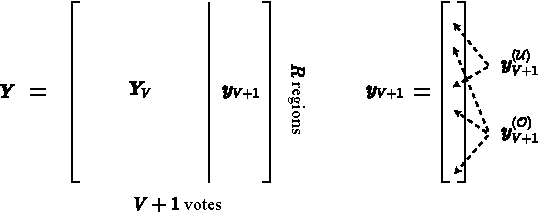
\includegraphics{pdk-structure.pdf}
	\caption{
		Decomposition of the vote matrix~$\vY$ into the fully observed \emph{sub-matrix}~$\vY_V$ and the new vote~$\vy_{V+1}$, whose results arrive sequentially.
		The~$(V+1)$ votes are chronologically ordered and the~$R$ regions are arbitrarily ordered.
	}
	\label{pdk:fig:structure}
\end{figure}

To predict the missing entries of~$\vy^{(\Ubs)}_{V+1}$,~\citet{etter2016online} use standard matrix factorization with alternating least-squares (ALS) to minimize the non-convex loss based on the Frobenius norm
\begin{equation}
	\label{pdk:eq:matrix_factorization}
	\min_{\vA, \vB} \left\Vert \vY^{(\Obs)} - \rnd{\vA\vB^T}^{(\Obs)} \right\Vert_F,
\end{equation}
where~$\vA \in \mathbf{R}^{R \times D}$ and~$\vB \in \mathbf{R}^{V \times D}$ are two matrices of latent dimension~$D \in \mathbf{N}_{>0}$, and where superscript~$(\Obs)$ denotes that, in this case, only the observed entries are kept.
With ALS, each iteration is expensive, and there are neither convergence guarantees nor explicit convergence rates~\cite{bell2007scalable, koren2009matrix}.
According to the Eckart-Young-Mirsky Theorem~\citep{eckart1936approximation}, the optimal solution to Equation~\eqref{pdk:eq:matrix_factorization} is the SVD, which is only computable if~$\vY^{(\Obs)}=\vY$.
We devise a more effective algorithm motivated by the special structure of this collaborative filtering problem\cite{etter2016online}.

\subsection{Algorithm}

Our algorithm works in four steps:
First, the fully-observed sub-matrix~$\vY_V$ is decomposed using SVD as
\begin{equation}
	\label{pdk:eq:svd}
	\vY_V \approx \vU \vSigma \vV\T,
\end{equation}
where the diagonal matrix~$\vSigma \in \mathbf{R}^{D \times D}$ stores the singular values, and where the matrices~$\vU \in \mathbf{R}^{R \times D}$ and~$\vV \in \mathbf{R}^{V \times D}$ store the~$D$ left and right singular vectors with the highest singular values, respectively.

Second, we compute the projection of the regions into the vote space as
\begin{equation}
	\label{pdk:eq:projection}
	\vX = \vY_V \vV = \vU \vSigma,
\end{equation}
where the matrix~$\vX \in \mathbf{R}^{R \times D}$ stores~$D$-dimensional representations of the regions.
We explore these representations in more detail in Section~\ref{pdk:sec:experiments}.
These two steps are performed offline, \textit{i.e.}, they are performed once.

Third, we use the observed results of a new vote~$\vy_{V+1}$ and the representations of observed regions in~$\vX$ to fit a GLM~$p$.
We find the maximum likelihood estimate~$\vw_* \in \mathbf{R}^D$ by minimizing the regularized negative log-likelihood of model~$p$ in Equation~\eqref{pdk:eq:glm}, with regularization parameter $\lambda \in \mathbf{R}$,
\begin{equation}
	\label{pdk:eq:log_likelihood}
	\ell_p(\vw ; \vX, \vy_{V+1}) = -\sum_{r \in \Obs} \log p(y_{r,V+1} \given \vw, \vx_r) + \lambda \| \vw \|_2^2,
\end{equation}
where $y_{r,V+1} \in \mathbf{R}$ is the result of the~$r$-th (observed) region, and~$\vx_r \in \mathbf{R}^D$ is the~$r$-th row of the representation matrix~$\vX$ corresponding to the representation of the~$r$-th region.

Finally, we predict the unobserved regions of the new vote~$\vy_{V+1}^{(\Ubs)} \in \mathbf{R}^{\vert \Ubs \vert}$ as the mean of the GLM~$p$ using the link function~$g$.
From the optimal parameters~$\vw_*$, we compute
\begin{equation}
	\label{pdk:eq:prediction}
	\vy^{(\Ubs)}_{V+1} := g^{-1}\left(\vX^{(\Ubs)} \vw_*\right),
\end{equation}
where~$\vX^{(\Ubs)} \in \mathbf{R}^{\vert \Ubs \vert \times D}$ are the representations of the unobserved regions.
The prediction for the national outcome is then the average of $\vy_{V+1}^{(\Obs)}$ and $\vy_{V+1}^{(\Ubs)}$, weighted by the population of each region $r$.
We summarize these steps in Algorithm~\ref{alg:algorithm}.

\begin{algorithm}
	\caption{\textsc{SubSVD-GLM}}
	\label{alg:algorithm}
	\begin{algorithmic}[1]
		\Input Sub-matrix~$\vY_V$, partial results~$\vy_{V+1}$, and GLM~$p$.
		\Output Prediction of unobserved results~$\vy_{V+1}^{(\Ubs)}$.

		\State Decompose $\vY_V \approx \vU \vSigma \vV\T$. \Comment{Equation~\eqref{pdk:eq:svd}}
		\State Project $\vX = \vU \vSigma$. \Comment{Equation~\eqref{pdk:eq:projection}}
		\State Optimize $\vw_* = \argmin_{\vw} -\ell_p(\vw ; \vX, \vy_{V+1})$. \Comment{Equation~\eqref{pdk:eq:log_likelihood}}
		\State Predict $\vy^{(\Ubs)}_{V+1} = g^{-1}\left(\vX^{(\Ubs)} \vw_*\right)$. \Comment{Equation~\eqref{pdk:eq:prediction}}

	\end{algorithmic}
\end{algorithm}

To predict the outcomes of referenda and elections, we use the GLMs described in Table~\ref{pdk:tab:glm}.
For referenda, we use univariate Gaussian and Bernoulli likelihoods.
For elections, we use multivariate Gaussian and categorical likelihood.
When a univariate Gaussian likelihood is used, the optimal parameters~$\vw_*$ can be learned (step 3 of Algorithm~\ref{alg:algorithm}) in closed form with least-squares
\begin{equation}
	\label{pdk:eq:least_squares}
	\vw_* = \rnd{\vX^{(\Obs)\intercal} \vX^{(\Obs)} + \lambda \vI_D }^{-1}\vX^{(\Obs)\intercal} \vy^{(\Obs)}_{V+1},
\end{equation}
where~$\vX^{(\Obs)} \in \mathbf{R}^{\vert \Obs \vert \times D}$ are the representations of the observed regions,~$\vy^{(\Obs)}_{V+1} \in \mathbf{R}^{\vert \Obs \vert}$ are the observed entries of the new vote, and~$\vI_D$ is a~$D$-dimensional identity matrix.
In general, we make the algorithm more efficient by reusing the optimal parameters~$\vw_*$ learned with~$\vert \Obs \vert$ observations when new observations arrive.

Although this algorithm is intuitive, considering the particular structure shown in Figure~\ref{pdk:fig:structure}, its general performance is not obvious.
In standard matrix factorization, defined in Equation~\eqref{pdk:eq:matrix_factorization}, both~$\vA$ and~$\vB$ are learned together.
Our algorithm fixes~$\vA$ to be equal to~$\vX = \vU \vSigma$, at the expense of adding some constraints, but with the benefit of computational complexity and identifiability gains.
In terms of identifiability, our regularized negative log-likelihood is strictly convex, which now guarantees a unique global optimum.
To limit computational cost, we factorize the matrix~$\vY_V$ only once and reuse its decomposition for each new observation(s) in~$\vy_{V+1}$.
Computing one SVD has complexity~$O(RD^2)$, as typically~$D \leq R$.
The optimization procedure (step 3) can be performed efficiently, \textit{e.g.}, in~$ O(n (\vert \Obs \vert D + D^3))$ for~$n$ iterations of Newton's method.
With a univariate Gaussian likelihood, computing the least-squares solution has asymptotic complexity~$O(\vert \Obs \vert D^2 + D^3)$, which is dominated by the~$\vert \Obs \vert D^2$ term, as typically~$D < \vert \Obs \vert$.
Finally, predicting unobserved values is only a (function of a) matrix-vector multiplication of complexity~$O(\vert \Ubs \vert D)$.

Elections are more complex than referenda because they have categorical outcomes.
Let~$K$ be the number of possible outcomes (for example~$K$ political parties).
The vote result matrix becomes a tensor~$\vY_V \in \mathbf{R}^{R \times V \times K}$.
To apply our algorithm, we concatenate the results of each party to collapse the last dimension.
This yields a matrix~$\vY_V \in \mathbf{R}^{R \times VK}$ that can be decomposed using SVD to obtain representations of regions (steps 1 and 2).
For an election, the regional results are stored in a matrix \mbox{$\vy_{V+1} \in \mathbf{R}^{R \times K}$}, and we use multivariate Gaussian or categorical likelihoods in the GLM to model the multiple outcomes (steps 3 and 4).

% TODO: Add sentences about how to obtain final prediction by aggregating observed results and predicted results.
% TODO: Mention that categorical distribution is equivalent to the multinomial distribution with N=1 (one trial).
% TODO: Define the softmax function in a footnote.
% TODO: Mention that we can include a bias term in the weights to learn the offset.

\subsection{Probabilistic Interpretation}

Voting data have the special property that the sum of all possible outcomes in a given region is equal to 1.
The outcome~$p \in [0, 1]$ of a referendum is the probability~$p$ that it is accepted (and the probability~$1-p$ that it is rejected).
The suffrage~$\vp \in [0, 1]^K$ obtained by~$K$ political parties in an election describes the probability mass function~$p(k)$ that the~$k$-th party is elected.
As a result, we provide a probabilistic interpretation of outcomes of referenda and elections.

Let~$P_{rv}^{(i)} \sim \DBernoulli{p_{rv}}$ be a random variable representing the vote cast by voter~$i$ in region~$r$ on referendum~$v$.
As voting is anonymous, we do not observe individual votes, rather the average vote in each region
\begin{equation*}
	\frac{1}{N_r} \sum_{i=1}^{N_r} P_{rv}^{(i)},
\end{equation*}
where~$N_r$ is the number of voters in region~$r$, and whose expectation is $p_{rv}$.
By decomposing the result matrix~$\vY = \vA \vB\T$ as in Equation~\eqref{pdk:eq:matrix_factorization}, we posit that the parameter of the random variables describing individual voters is a product of latent features of regions and votes~$p_{rv} = \va_r\T \vb_v$, with~$\va_r, \vb_v \in \mathbf{R}^D$.
In Equation~\eqref{pdk:eq:svd} and Equation~\eqref{pdk:eq:projection}, our algorithm learns the latent features of the regions~$\va_r = \rnd{\vU \vSigma}_r = \vx_r$ from historical data.
In Equation~\eqref{pdk:eq:log_likelihood}, it learns the latent features of the votes~$\vb_v = \argmin_{\vb} -\ell_p(\vb ; \vX, \vy_v)$ as the parameters of a GLM~$p$.

So far, we have considered that each region has the same number of voters.
If we have access to data about the number of voters in each region (\textit{e.g.}, the number of valid votes, the number of eligible voters, or the population), we can include this information by replacing the regularized log-likelihood in~\eqref{pdk:eq:log_likelihood} by
\begin{equation}
	\label{pdk:eq:weighted}
	-\ell_p(\vw ; \vX, \vy_{V+1}) = \sum_{r \in \Obs} N_r \log p(y_{r,V+1} \given \vw, \vx_r) + \lambda \Vert \vw \Vert_2^2,
\end{equation}
where $N_r \in \mathbf{R}$ is a count related to the number of voters in region~$r$.
We refer to the variation of the algorithm that uses this log-likelihood as \textit{weighted}.
We refer to the variation of the algorithm that uses the log-likelihood in~\eqref{pdk:eq:log_likelihood} as \textit{unweighted}.
A similar argument can be trivially made for elections by letting~$P_{rv}^{(i)} \sim \DCategorical{\bm{p}_{rv}, K}$ be a random variable describing the vote cast by voter~$i$ in region~$r$ on vote~$v$ for $K$ political parties.

\subsection{Limitations}

By design, our approach suffers from the cold-start problem of collaborative filtering~\cite{koren2009matrix}.
We can make predictions only when at least one past observation is available, \textit{i.e.}, when~$\vert \Obs \vert = 1$.
To bypass this problem,~\citet{etter2016online} include features of the regions, such as the geographical location, the population size, and the elevation, and features of the votes, such as the voting recommendation by political parties.
These features are, however, not systematically and programmatically available, making it difficult to use them in a real-world system such as the one we describe in Section~\ref{pdk:sec:depsys}.

Our approach also makes the hypothesis that regional and vote representations are static over time.
In particular, the algorithm learns the regional representations over the whole training set.
The latest results might, however, provide more information than older results.
To bypass this problem, we could weigh the SVD by using a sliding window or by exploiting a temporal SVD algorithm~\cite{bamler2017dynamic} to capture the dynamics of the voting process.

% Other sources of data, \textit{e.g.}, polling data, could be used to make predictions prior to a vote.
% However, the business model of polling agencies often solely relies on their data, which prevents them from sharing their datasets.
% Textual data, for example extracted from the actual law proposal or from parties documents would also constitute valuable data.
% But the specificity of legal text makes it difficult to process and exploit such datasets, and we keep this direction as future work.

%! TEX root = ../thesis.tex
\section{Experimental Results}%
\label{pdk:sec:experiments}

\begin{table}
	\centering
	\caption{
		Description of datasets used in our experiments.
	}
	\label{pdk:tab:datasets}
	\begin{tabular}{lllrrrr}
		\toprule
		Country     & Type   & Region   & $R$             & $V$            & $K$ & Period     \\
		\midrule

		% Switzerland   & Binary      & Municipality & \numprint{2196} & \numprint{330} & -- & 1981--2020 \\
		% United States & Binary      & State        & \numprint{50}   & \numprint{11}  & -- & 1976--2018 \\
		Switzerland & Binary & Munic.   & \numprint{2196} & \numprint{330} & --  & 1981--2020 \\
		U.S.        & Binary & State    & \numprint{50}   & \numprint{11}  & --  & 1976--2016 \\
		Germany     & Categ. & State    & \numprint{16}   & \numprint{6}   & 5   & 1990--2009 \\
		Germany     & Categ. & District & \numprint{538}  & \numprint{5}   & 5   & 1990--2005 \\

		\bottomrule
	\end{tabular}
\end{table}

We evaluate our algorithm on the four datasets\footnote{The data and the code are available on \href{https://www.github.com/indy-lab/submatrix-factorization}{github.com/indy-lab/submatrix-factorization}.} described in Table~\ref{pdk:tab:datasets}.
The outcomes for the Swiss referenda and for U.S.\ presidential elections are binary.
For Switzerland, this corresponds to the referendum being accepted or rejected.
For the U.S.\, this corresponds to one presidential candidate being elected over the other.
The outcomes for the German legislative elections are one of five categories, corresponding to five political parties.

For the binary datasets, \textit{i.e.}, for Switzerland and for the U.S., we use a GLM~$p$ with univariate Gaussian and Bernoulli likelihoods.
As data about the number of valid votes and about population counts are available for these two datasets, we use a likelihood with weighting, as defined in~\eqref{pdk:eq:weighted}.
For the categorical datasets, \textit{i.e.}, for Germany, we use a GLM with multivariate Gaussian and categorical likelihoods.
As data about population counts were not available in this case, we use a likelihood without weighting, as defined in in~\eqref{pdk:eq:log_likelihood}.

\subsection{Evaluation}

For each dataset, we find the best hyperparameters using the training set only. %, as explained in details in Appendix~\ref{pdk:app:experimental_setting}.
To evaluate the performance of our algorithm, we compute the mean absolute error (MAE) and the accuracy on the national results.

We first describe the error metrics used for the binary outcome case then extend them for multiple outcomes, \textit{e.g.}, when different parties can be voted.
Let $\vy^* \in \mathbf{R}^R$ be the true regional results and let $\vy \define \vy_{V+1} \in \mathbf{R}^R$ be a prediction.
The true national outcome $y^* \in \mathbf{R}$ is defined as
\begin{equation*}
	y^* \define \frac{1}{N} \sum_{r \in [R]} N_r y_r^*,
\end{equation*}
where $N = \sum_{r \in [R]} N_r$ is the total number of voters.
The predicted national outcome $y \in \mathbf{R}$ is defined as
\begin{equation*}
	\label{pdk:eq:prediction}
	y \define \frac{1}{N}\left( \sum_{r \in \Ubs} N_r y_r + \sum_{r \in \Obs} N_r y_r^* \right),
\end{equation*}
where the prediction $y_r$ in some observed region~$r \in \Obs$ equals the true outcome $y_r^*$.
Then, the MAE and the accuracy of the national prediction are computed as
\begin{align}
	\mae(y, y^*)         & = \vert y - y^* \vert, \label{pdk:eq:mae}                                                                                  \\
	\textrm{Acc}(y, y^*) & = \Indic{y \geq 0.5 \textrm{ and } y^* \geq 0.5} \nonumber + \Indic{ y < 0.5 \textrm{ and } y^* < 0.5}, \label{pdk:eq:acc}
\end{align}
where $\Indic{\cdot}$ is the indicator function.

The MAE enables us to evaluate how far a predictor is from the exact percentage value, whereas the accuracy enables us to evaluate if the outcome is predicted correctly.
For $K$ outcomes, the true and the predicted outcomes are vectors $\vy^* \in [0, 1]^K$ and $\vy \in [0, 1]^K$, respectively, and the MAE in~\eqref{pdk:eq:mae} is simply the $\ell_1$-norm of the difference between the two vectors.
As the accuracy is not defined for multiple outcomes, we compute the average displacement (or Spearman's footrule)~\cite{diaconis1977spearman}.
Let \mbox{$p: [K] \rightarrow [K]$} be a permutation map from a party to its rank for the predicted order, and let \mbox{$p^*: [K] \rightarrow [K]$} be a permutation map for the true order.
The average displacement is then computed as
\begin{equation*}
	D(p, p^*) = \frac{1}{K} \sum_{k=1}^K \vert p(k) - p^*(k) \vert.
\end{equation*}
This measures the average position shift between the true rank and the predicted rank of each party.

We train our algorithm on data up to vote $V$ and make predictions on vote $V+1$ to evaluate our algorithm.
To simulate a real setting where results arrive sequentially, we incrementally add regions to the set of observed regions $\Obs$ and average the MAEs on several reveal orders to obtain error bars.
Current political forecasting methods for real-time estimation of the outcomes (\textit{e.g.}, by media outlets) rely mostly on weighted averages of the regional results on the day of the vote.
More sophisticated methods (developed, \textit{e.g.}, by polling agencies) can also be used, but their technical details are not available.
Hence, we compare our algorithm against weighted averaging as a baseline.
For the binary classification task, we also compare against standard matrix factorization (MF) trained with alternating least squares, as proposed by~\citet{etter2016online} and as formulated in Equation~\eqref{pdk:eq:matrix_factorization}.
For the multiple outcome task, we restrict our comparison to weighted averaging.

\subsection{Swiss Referenda}
\label{pdk:sec:swiss_referenda}

We collect a dataset of $V=330$ referenda in $R=2196$ municipalities (the regions are here the municipalities) between 1981 and 2020.
We start with a training set of $V=300$ votes and report the average performance on the next 26 votes with $100$ reveal orders each.
As several votes can occur on the same day, we make sure that only past votes are used in the training set.
In Section~\ref{pdk:sec:depsys}, we analyze in depth the last four votes (two votes on two dates) for which we have real, sequential data.
The best combination for the Bernoulli likelihood is $\lambda = 0.01 $ and $D = 25$.
% The ranges of hyperparameters are given in Appendix~\ref{app:ch}, and the best combination for the Bernoulli likelihood is $\lambda = 0.01 $ and $D = 25$.

In Figure~\ref{pdk:fig:ch_results}, we show the MAE and the accuracy of our algorithm to predict national results from partial municipal results.
The two likelihoods used for the GLM provide equal performance, and we report only the performance of the Bernoulli likelihood for clarity.
In terms of MAE (top), MF outperforms the weighted average baseline and our algorithm outperforms MF for every number of observed regions from 1 to 1000.
The difference becomes marginal when more than 1000 results are observed, which suggests that a good approximation of the national result can be obtained by simply averaging the observed results when more than 50\% of the results have arrived.
Nevertheless, in this synthetic setting (the reveal order is randomized) our approach gains only one percentage point at best over the baseline.
In Section~\ref{pdk:sec:depsys}, we will show that the gain becomes substantial with real data, \textit{i.e.}, with the actual reveal order.
In terms of accuracy (bottom), our algorithm predicts the final outcome with 95\% accuracy with 10 observed regions only, outperforming the two baselines by 5 percentage points.
The accuracy of our algorithm reaches 100\% after observing 200 municipal results, \textit{i.e.}, after observing 10\% of all municipalities.

\begin{figure}
	\centering
	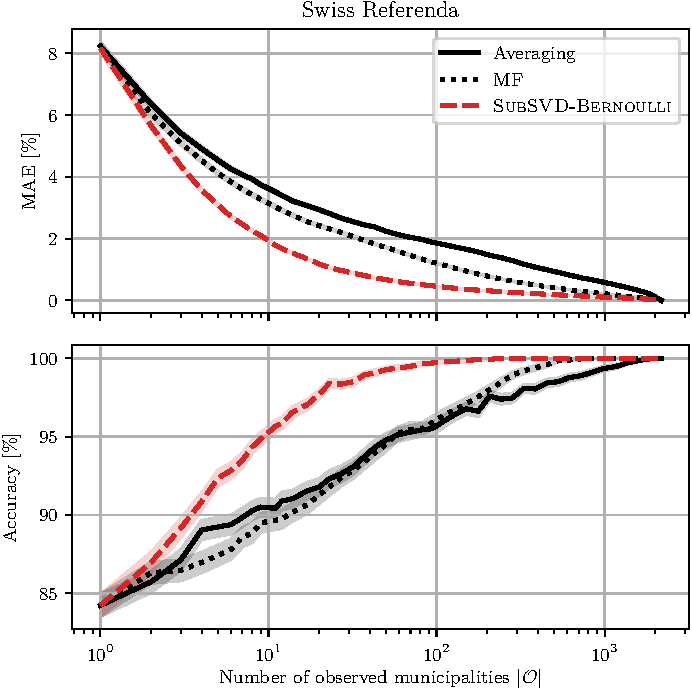
\includegraphics{pdk-ch-results.pdf}
	\caption{MAE (top) and accuracy (bottom) averaged over 26 Swiss referenda and 100 reveal orders each.}
	\label{pdk:fig:ch_results}
\end{figure}

We explore the patterns in the feature matrix $\vX = \vU \vSigma$ obtained from~\eqref{pdk:eq:projection}.
In Figure~\ref{pdk:fig:ch_svd}, we plot the first two columns of $\vX$, \textit{i.e.}, a projection of the municipalities on the first two singular vectors of the vote representation.
This plot, popularized by~\citet{etter2014mining}, shows two clear clusters of municipalities corresponding to their language.
It also exhibits the infamous \textit{Röstigraben}, a cultural separation between French-speaking municipalities and German-speaking municipalities.
% \footnote{Literally the {\em hash-brown ditch}. It refers to the protective moat set up by the hard-working, frugal, and well-organized Swiss Germans to keep hard-drinking French-speaking leftist rascals at bay.}
In addition, we show in Figure~\ref{pdk:fig:ch_tsne} a projection of the result matrix $\vY$ by using t-SNE~\citep{maaten2008visualizing}.
The language separation is also clearly visible, with French-speaking municipalities on the left of the plot and German-speaking municipalities on the right.
The group of municipalities are further subdivided into smaller clusters corresponding to the canton (states of the Swiss confederation) that they belong to.
Most cantons are uni-lingual in Switzerland, but a few are bilingual.
The most notable among them is Wallis, and interestingly enough, we observe that it is separated into two distinct clusters.
The French-speaking municipalities in Wallis are closer to other French-speaking municipalities, and vice versa for the German-speaking municipalities.
The municipalities of the only Italian-speaking canton, Ticino, form their own cluster.

\begin{figure}
	\centering
	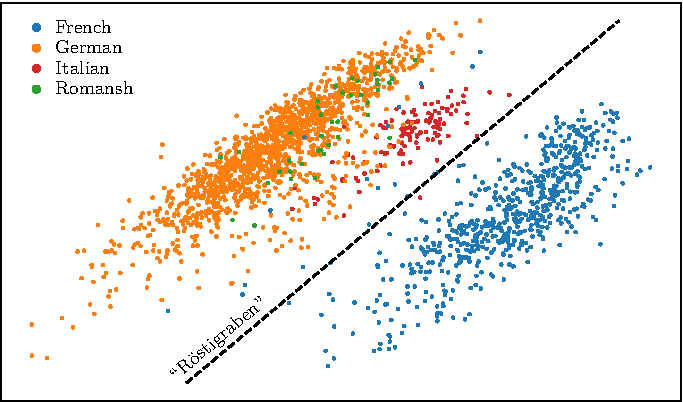
\includegraphics{pdk-ch-svd.pdf}
	\caption{
		Projection of Swiss municipalities on the first two singular vectors of referendum matrix $\vY$.
		Municipalities are colored according to their language.
	}
	\label{pdk:fig:ch_svd}
\end{figure}

\begin{figure}
	\centering
	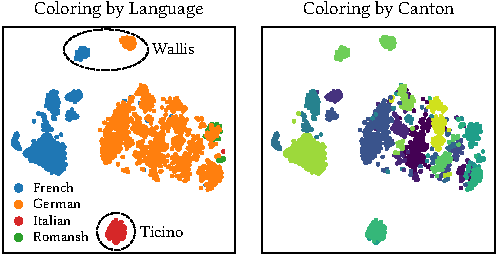
\includegraphics{pdk-ch-tsne.pdf}
	\caption{
		Projection of Swiss municipalities from referendum matrix $\vY$ with t-SNE.
		(Left) Municipalities are colored according to their language.
		(Right) Municipalities are colored according to their canton (26 cantons).
		The bilingual canton of Wallis is split into two clusters.
		The only Italian-speaking canton of Ticino is isolated from the other clusters.
	}
	\label{pdk:fig:ch_tsne}
\end{figure}

\subsection{U.S.\ Presidential Election}

The U.S.\ presidential election takes place every four years.
We obtain a dataset about the state-level ballots between 1976 and 2016~\citep{mit2017us}.
In the spirit of Nate Silver's \textit{FiveThirtyEight}~\citep{silver2008pollster}, we evaluate the performance of our algorithm at predicting the result of the U.S.\ presidential election in 2016.
The U.S.\ presidential election relies on the electoral-college system, which adds one level of complexity to the prediction because (1) the state-level results are quantized to an integer number of delegates and (2) the candidate who wins the majority of votes in a state wins all the delegates of that state.
This (non-linear) winner-take-all rule requires further modeling assumptions and is out of the scope of this work.
Instead, we focus on predicting the results of the popular vote.

We transform the outcome of the election into a binary outcome of Democratic candidate and Republican candidate.
In all these elections, the results of other parties, \textit{e.g.}, the Green party and independent candidates, are insignificant compared to the two major U.S.\ parties.
This dataset contains the results of $V = 11$ votes in $R = 51$ regions (50 states and the District of Columbia) between 1976 and 2016.
As the number of votes is small, we train our algorithm on all votes up to 2012 ($V = 10$) to set the sub-matrix $\vY_V$, and we predict the state-level results and the national results of the 2016 election.
We report the averaged performance on $10000$ random reveal orders.
The best combination for the Bernoulli likelihood is $\lambda = 0.01 $ and $D = 7$.
% The ranges of hyperparameters are given in Appendix~\ref{app:us}, and the best combination for the Bernoulli likelihood is $\lambda = 0.01 $ and $D = 7$.

In Figure~\ref{pdk:fig:us_results}, we show the MAE and the accuracy of our algorithm in predicting this election.
The two likelihoods used for the GLM provide equal performance, and we report only the performance of the Bernoulli likelihood for clarity.
In terms of MAE (top), our algorithm and MF outperform the weighted average baseline after observing the results in two regions.
In terms of accuracy (bottom), our algorithm outperforms both MF and the weighted average for any number of observation.
All models have an accuracy of 41\% after observing the result of one region.
This is because the Democratic candidate won in 21 of 51 regions (41\%) and won the popular vote.

\begin{figure}
	\centering
	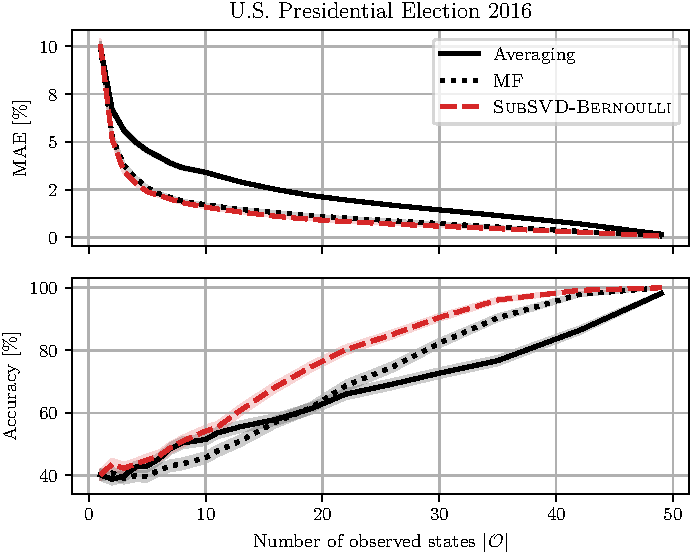
\includegraphics{pdk-us-results.pdf}
	\caption{MAE (top) and accuracy (bottom) of the popular vote of the U.S.\ presidential election in 2016.}
	\label{pdk:fig:us_results}
\end{figure}

\subsection{German Legislative Election}

German legislative elections take place every four years.
We obtain two datasets~\cite{norsk2020germany} of regional results with $R=16$ states (1990--2009) and $R=538$ districts (1990--2005).
After 2005 (for the districts) and 2009 (for the states), the data are regrettably not publicly available any longer.
We keep $K = 5$ political parties, corresponding to the five major parties in Germany\footnote{CDU/CSU (christian democracy), SPD (social liberalism), FDP (conservative liberalism), the Green party (ecological), and the Left party (radical left).} for which we have data over the whole period.
The datasets cover $V=6$ votes for state-level results and $V=5$ for district-level results.
As there are multiple outcomes, we use a categorical likelihood to predict the results of the five parties.

For the state-level results, we train our algorithm on all votes up to 2005 ($V = 5$) to set the sub-matrix $\vY_V$, and we predict the national results of the 2009 election.
For the district-level results, we train our algorithm on all votes up to 2001 ($V = 4$), and we predict the national results of the 2005 election.
In Figure~\ref{pdk:fig:de_results}, we show the performance of our algorithm in predicting these two elections.
For both datasets, our algorithm outperforms the baseline already after a small number of observations.
The performance for the prediction of the national results when using the fine-grained district-level results is better than when using coarser-grained state-level results.
Remarkably, after observing the results in 10 districts (Figure~\ref{pdk:fig:de_results}, top right), \textit{i.e.}, approximately the average number of districts per state, the MAE reaches 1\%, which is four times better than the MAE obtained after predicting the national outcome from one state (Figure~\ref{pdk:fig:de_results}, top left).
A similar observation can be made for the average displacement.
This suggests that the finer the level of granularity of regions is, the better the predictive performance is, even if the observed results are obtained from the same number of voters.

\begin{figure}
	\centering
	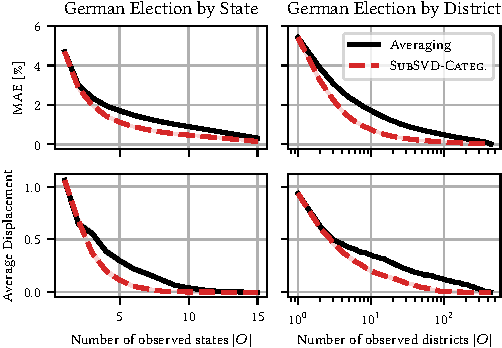
\includegraphics{pdk-de-results.pdf}
	\caption{MAE (top) and average displacement (bottom) of German legislative elections at state level in 2009 (left) and district level in 2005 (right).}
	\label{pdk:fig:de_results}
\end{figure}

Like with Switzerland in Section~\ref{pdk:sec:swiss_referenda}, we explore the representations of the regions contained in the feature matrix $\vX$ for Germany.
In Figure~\ref{pdk:fig:de_svd}, we plot the first two columns of $\vX$, \textit{i.e.}, a projection of the districts on the first two singular vectors of the vote representations.
We color the points according to the first party elected in the corresponding districts (left).
With no exception, either the CDU/CSU or the SPD is elected.
The two clusters are each separated in half:
The districts on the right side of their cluster vote in majority for the CDU/CSU.
For the lower cluster, those districts also belong to Southern Germany.
The districts on the left side of this cluster (which vote in majority for the SPD) belong to North-Western Germany.

\begin{figure}
	\centering
	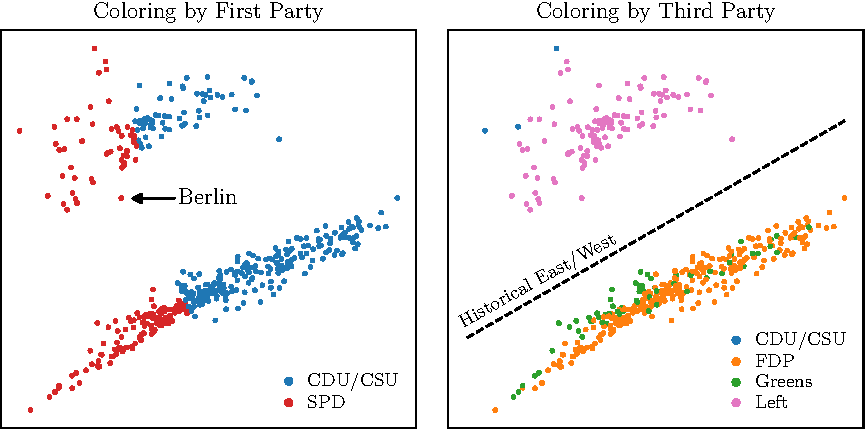
\includegraphics{pdk-de-svd.pdf}
	\caption{
		Projection of German district on the first two singular vectors of election matrix $\vY$.
		(Left) Districts are colored according to the first party elected in each of them.
		(Right) Districts are colored according to the third party elected.
		This coloring reveals the historical East/West separation.
	}
	\label{pdk:fig:de_svd}
\end{figure}

The CDU/CSU and the SPD have the top two ranks in all districts.
Therefore, it is interesting to color the points according to the party in third place.
This clearly separates the two clusters.
The cluster at the top corresponds to the Left party.\footnote{The three exceptions with CDU/CSU voted the Left party in second place.}
The top cluster contains only districts that belong to historical East Germany (formerly the GDR, before the reunification in 1990), such as Potsdam, Leipzig, and Dresden.
The cluster at the bottom corresponds to the Green party and the FDP and contains only districts that belong to historical West Germany (the former BDR), such as Frankfurt, Munich, and Hamburg.
Interestingly, Berlin lies in the cluster that corresponds to historical East Germany, but seems slightly isolated.

%! TEX root = ../thesis.tex
\section{Deployed System}%
\label{pdk:sec:depsys}

We deploy a Web platform, called Predikon\footnote{The platform is available on \href{http://www.predikon.ch}{www.predikon.ch}.}, to provide real-time predictions for Swiss referenda (see Appendix~\ref{app:sec:predikon}.
Four Sundays a year, Swiss citizens are called on to vote on at least one item in a referendum.
These items can cover a broad range of topics, from joining the European Union to subsidizing railways and roads, from banning the use of fossil fuels to cutting taxes, and even forbidding Swiss farmers to remove horns from cows and goats.
A month prior to a referendum vote day, eligible voters receive official ballots, together with useful documentation.
To cast their vote, they can either send their ballot by post or bring it to the ballot office on the referendum vote day, up to 11:59am.
Starting at 12pm, each municipality is in charge of counting both the remote ballots and the ballots they collected on the same day.
Once they have finished counting, they report the result to their canton whose administration communicates the official count.

\subsection{Implementation Details}

In 2019, the Swiss Federal Statistical Office released a public API to access vote data, both historical and real-time, for all municipalities in a standardized format~\cite{confederation2020open}.
This enabled us to obtain sequential results in all municipalities on the referendum vote days and made it possible to use our algorithm to predict the outcome of referenda starting at 12pm.
We use the dataset described in Table~\ref{pdk:tab:datasets} for Switzerland, which contains~$R = 2196$ municipalities.
We predict the outcome of twelve items between February 9, 2020, and March 7, 2021.
We summarize these items in Table~\ref{pdk:tab:real_votes}.
On average, the turnout is 53.3\% and 2.8 million valid ballots are counted for each referendum.

\begin{table}
	\centering
	\caption{
		True outcome $y^*_{\textrm{nat}}$, earliest prediction $y_{\textrm{nat}}$, and absolute difference $\Delta = \vert y^*_{\textrm{nat}} - y_{\textrm{nat}} \vert $ for referenda with real data.
	}
	\label{pdk:tab:real_votes}
	\begin{tabular}{llrrr}
		\toprule
		Date         & Item                                & $y^*_{\textrm{nat}}$ [\%] & $y_{\textrm{nat}}$ [\%] & $\Delta$ \\
		\midrule

		Feb 9, 2020  & More Affordable Housing             & 42.97                     & 41.57                   & 1.40     \\
		             & Ban of Sexual Discrimination        & 63.03                     & 62.95                   & 0.08     \\
		Sep 27, 2020 & Moderate Immigration                & 38.35                     & 38.53                   & 0.18     \\
		             & Hunting Act                         & 48.07                     & 47.54                   & 0.53     \\
		             & Tax Deduction of Childcare Expenses & 36.77                     & 35.58                   & 1.19     \\
		             & Paternity Leave                     & 60.27                     & 59.33                   & 0.94     \\
		             & New Fighter Aircrafts               & 50.16                     & 51.29                   & 1.13     \\
		Nov 29, 2020 & Responsible Businesses              & 50.73                     & 50.13                   & 0.60     \\
		             & Ban on Financing War Material       & 42.55                     & 41.91                   & 0.64     \\
		Mar 7, 2021  & Ban on Full Face Coverings          & 51.21                     & 50.80                   & 0.41     \\
		             & e-ID Act                            & 35.64                     & 38.03                   & 2.39     \\
		             & Trade Agreement with Indonesia      & 51.65                     & 51.54                   & 0.11     \\

		\bottomrule
	\end{tabular}
\end{table}

For a vote~$V+1$, we use the historical data up to vote~$V$ to learn the feature matrix~$\vX$ from the sub-matrix~$\vY_V$.
For example, for February 9, 2020, we train the model using~$V = 328$ votes and we predict the results of the two referenda on that date.
We use a Bernoulli likelihood to define our GLM with~$D=25$ latent dimensions and a regularization factor~$\lambda=0.01$.
We fetch municipal results from the API every minute\footnote{Schedule suggested by the Swiss Federal Statistical Office.}.
If new results are available, we learn the optimal parameters~$\vw_*$ by optimizing the negative log-likelihood using Newton's method, and we predict the unobserved municipal results as $\vy_{V+1}^{(\Ubs)} = \sigma(X^{(\Ubs)} \vw_*)$.
Similar to Equation~\eqref{pdk:eq:prediction}, we predict the national outcome~$y_{\textrm{nat}} \in [0, 1]$ by aggregating our prediction of unobserved results~$\Ubs$ with the observed results~$\Obs$ as
\begin{equation*}
	y_{\textrm{nat}} = \frac{1}{N} \left( \sum_{r \in \Ubs} N_r^{(\Ubs)} y_{r, V+1}^{(\Ubs)} + \sum_{r \in \Obs} N_r^{(\Obs)} y_{r, V+1}^{(\Obs)} \right),
\end{equation*}
where~$N_r^{(\Ubs)}$ is the number of valid ballots in municipality~$r$ from the previous vote (used as proxy for the current vote),~$N_r^{(\Obs)}$ is the number of valid ballots in municipality~$r$ for the current vote, and~$N = \sum_{r \in \Ubs} N_r^{(\Ubs)} + \sum_{r \in \Obs} N_r^{(\Obs)}$ is the total number of valid ballots.
As the number of unobserved results~$\vert \Ubs \vert$ tends to 0 with time and the number of observed results~$\vert \Obs \vert$ tends to the total number of regions~$R$, the prediction for the national outcome~$y_{\textrm{nat}}$ converges to the true outcome~$y_{\textrm{nat}}^* \in [0, 1]$.

\subsection{Real-Time Predictions}

In Figure~\ref{pdk:fig:predictions}, we show eight examples of the evolution of our predictions (red line), together with the weighted averaging (black line), as a function of the progress of the ballot counting.
The ballot counting starts at 12pm and ends later in the afternoon, after all municipalities reported their results.
Looking at the trajectory of the weighted averaging, the jumps occurring at several steps correspond to the publication of the results of whole cantons, such as Wallis, and of large municipalities, such as the cities of Basel, Genera, Bern or Zurich.

Our first predictions are made at 12:01pm, using the results of 355 municipalities on average (16.2\% of all municipalities) representing 6.5\% of the total population.
For the twelve referenda, these predictions reach a mean absolute error of 0.8\% to the true outcome.
The largest error is made on the ``e-ID Act'', with a MAE of 2.39\%.
This could be due to the lack of historical votes related to digitalization in Switzerland leading to a vote embedding lying in an empty region of the ideological space.
The weighted average for the current count varies up to a difference of 7.3\%, whereas our predictions are qualitatively stable over time.
To provide a robust estimation of the final outcome, our algorithm takes advantage of the correlation across municipalities and votes.
Furthermore, our earliest predictions were always on the correct side of the 50\% threshold, \textit{i.e.}, it reached an accuracy of 100\% at predicting the acceptance or rejection of a referenda.

\begin{figure}
	\centering
	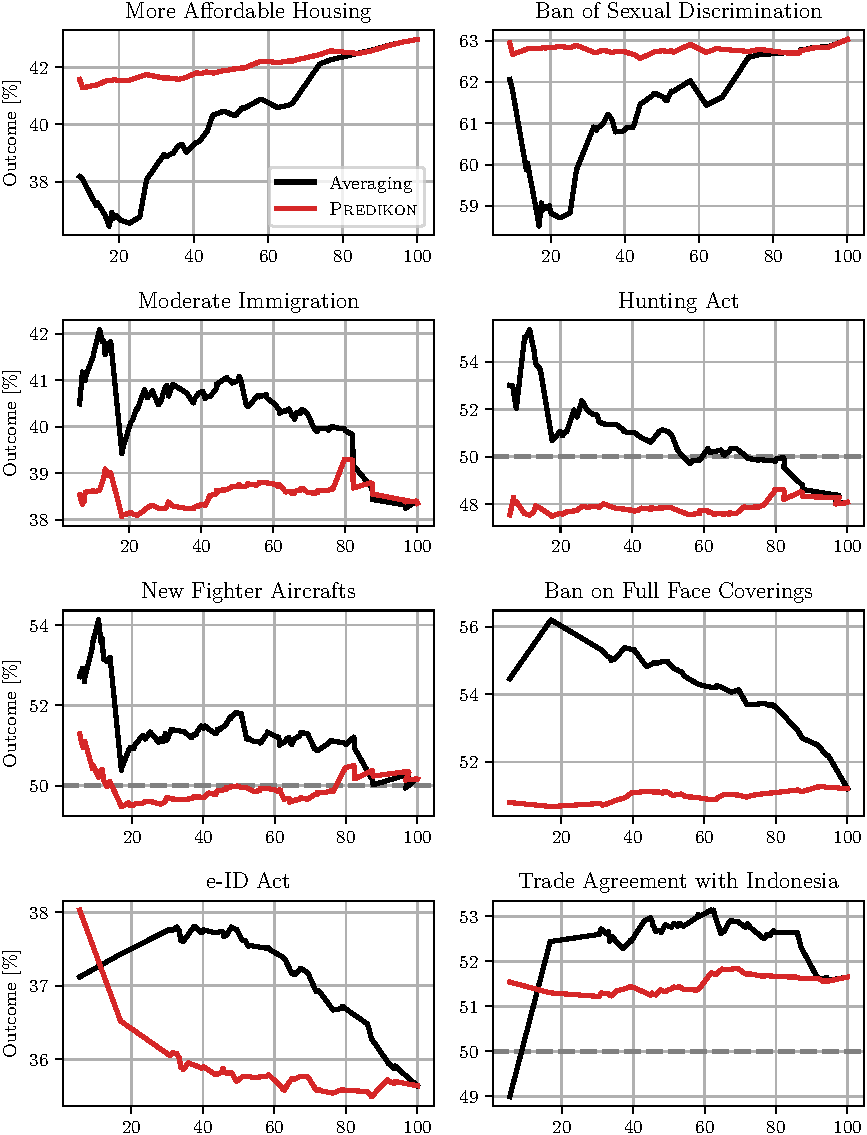
\includegraphics{pdk-predictions.pdf}
	\caption{
		Examples of evolution of predictions (red) and weighted averaging (black) on real, sequential data for the referenda between February 9, 2020, and March 7, 2021.
	}
	\label{pdk:fig:predictions}
\end{figure}

\section{Related Work}%
\label{sec:relwork}

We base the present paper on the work of~\citet{etter2014mining} and build on their approach proposed in~\cite{etter2016online}.
They combine matrix factorization and Gaussian processes (GP) to understand what features of the votes and of the municipalities contribute the most to the predictive performance.
They develop an expectation-maximization algorithm to learn both latent features and the GP parameters jointly.
They show that the geographical location of municipalities is the most important feature for making predictions, an aspect that is in part captured by the feature matrix $\vX$ of Equation~\eqref{eq:projection} in our algorithm and illustrated in Figure~\ref{fig:ch_svd}:
Municipalities that are geographically close tend to speak the same language.
They also show that they are able to make accurate predictions of Swiss referenda.
In comparison, our method is more efficient, as it learns the latent features of municipalities $\vX$ through singular value decomposition offline, and it learns the latent features of a vote through a GLM.
The GLM also provides more flexibility:
Our algorithm could conceivably be used to make prediction for other types of observations, \textit{e.g.}, count data, and works for non-binary outcomes.
We developed our algorithm with applicability in mind.
Our main goal was to make real-time predictions for Swiss referenda, with all the constraints that come with this problem.

The problem we address, \textit{i.e.}, predicting unobserved entries of a new column of a matrix from partial observations of that column, is most similar to the problem of missing-data imputation.
The use of SVD for data imputation has been studied in the context of genomics~\citep{troyanskaya2001missing,hastie1999imputing}.
In gene matrices, missing entries are common, and the authors propose an algorithm based on SVD to impute missing data.
Their algorithm iteratively computes the SVD of an approximation to the full matrix and predicts the missing values with a regression by using the non-missing values to refine the approximation.
An extensive literature review of predictive methods for data imputation is available in~\citet{bertsimas2017predictive}.
Incremental SVD revisions have been studied in the context of computer vision~\citep{brand2002incremental} and recommender systems~\citep{brand2003fast}.
In this latter work, the author proposes algorithms to compute the SVD of a matrix when new columns arrive sequentially and are corrupted by some noise (\textit{e.g.}, some entries are missing).
Their solution is equivalent to our \textsc{SubSVD-Gaussian} algorithm without regularization, \textit{i.e.}, $\lambda=0$, for which a closed form solution is provided in Equation~\eqref{eq:least_squares}.

A whole body of work in the political science community exists on election forecasting~\citep{lewis2005election}, \textit{i.e.}, predicting the outcome of an election before it happens.
The seminal work of~\citet{bean1948predict}, who first studied this problem in 1948, looked at using historical data to find U.S.\ states that were the most predictive of the national outcome.
Statistical models for election forecasting have since been developed in many contexts for Germany~\citep{tumasjan2011election}, France~\citep{belanger2004finding}, the U.K.~\citep{franch2013wisdom}, and the U.S.~\citep{rigdon2009bayesian,kennedy2017improving}.
The prediction of U.S.\ elections has been popularized by the blogger and statistician Nate Silver in 2008 as he predicted Barack Obama's victory in the Democratic Party primaries using a statistical model of historical data~\citep{blumenthal2008poblano}, and as he predicted Barack Obama's victory in the presidential election from polling data~\citep{silver2008pollster}.
In the computer science community, algorithms for election forecasting have also been developed using social media data in Denmark~\citep{kristensen2017parsimonious}, Finland~\citep{vepsalainen2017facebook}, the U.S.~\citep{choy2012us,ramteke2016election}, and the developing world~\citep{dwi2015twitter}.
To the best of our knowledge, except for the work mentioned at the beginning of this section, we are the first to study real-time outcome predictions of elections and referenda, and to deploy a system for making predictions of Swiss referenda in real-time.

%! TEX root = ../thesis.tex
\section{Summary}%
\label{pdk:sec:conclusion}

In this chapter, we have proposed an algorithm to predict national vote results from regional results that are observed sequentially.
Our approach learns a representation for each region by factorizing the sub-matrix of historical data and approximating the representation of a new vote as the optimal parameters of a generalized linear model.
The predictions for unobserved results are obtained through the link function of the GLM, and national predictions are obtained by aggregating observed and unobserved regional results.
We are able to predict both referenda with binary outcomes and elections with categorical outcomes.
We have shown that our approach outperforms the (weighted) average of partial results on three datasets of Swiss referenda, U.S.\ presidential elections, and German legislative elections.
We have explored the regional representations in their latent space and have shown that they capture ideological and cultural patterns.
Finally, we have deployed a Web platform to provide real-time vote predictions for Swiss referenda.
Our algorithm is able to predict the final outcome of four real votes with an absolute error of about 1\% after observing only 13\% of the ballots.

\paragraph{Perspective}

We plan to further develop our approach in three directions.
First, Bayesian inference in our generalized linear model would enable uncertainty quantification of our predictions in a principled way.
This could be beneficial for predictions, especially during the early counting phase.
Bayesian inference for GLMs has been widely studied in the literature~\citep{murphy2012machine}.
Second, our algorithm is capable of making predictions only with at least one observed regional result.
In the spirit of~\citet{etter2016online}, we plan to augment our algorithm with features from the vote and the municipalities to make predictions prior to referenda in Switzerland.
One limitation of their work lies in the lack of systematic availability of the features they include in their model.
In particular, every Swiss citizen receives documentation about each referendum.
These explanatory documents provide a valuable source of information about a vote, one that could be incorporated in a predictive model.
The actual text of the proposed laws would provide another source of relevant information.
Finally, by collecting the sequential order by which regional results arrive in Swiss referenda, we obtain data about the true reveal order.
We plan to explore whether the true sequential order can be exploited to learn the schedule by which results arrive and, therefore, further improve the earliest predictions.


% Acknowledge people who helped.
\begin{acks}
We thank Holly Cogliati-Bauereis, Vincent Etter, Julien Herzen, and the anonymous reviewers for careful proofreading and constructive feedback.
We thank Corinne Straub of the Swiss Federal Statistical Office for setting up the API and helping us understand their data.
\end{acks}

% Add bibliography.
\bibliographystyle{abbrvnat}
\bibliography{submatrix}

\newpage
\clearpage
\appendix
%! TEX root = ../thesis.tex
\section{Experimental Setting}
\label{app:experimental_setting}

We describe in details the experimental setting and the choice of hyperparameters.
As explained in Section~\ref{pdk:sec:experiments}, we evaluate the predictive performance of our models and of the baselines after observing a fraction of regional outcomes.
For each dataset, we use the training set as validation set to find the best hyperparameters from a range of possible values.
We preserve the temporal order of the data, and we use the first $V$ votes for training while testing on the next vote $V+1$.
This simulates a real setting where we use all available data prior to an election or referendum of interest.

For each test vote, we simulate several random reveal orders of regional results.
For the Swiss referenda, the U.S.\ presidential election, and the German parliamentary election by district, we simulate reveal orders on a logarithmic space.
This emphasizes the importance of early results, \textit{i.e.}, when a small number of results are available, in the prediction performance.
For the German parliamentary election by states, the number of regions is small enough ($R=16$) to simulate reveal orders on a linear space.

We evaluate the performance of our models and of the baselines with different combinations of the hyperparameters.
The hyperparameters in our method are the $\ell_2$-regularization parameter $\lambda$ and the number of dimensions $D$ of the latent factors.
We report in Table~\ref{pdk:tab:ranges} the ranges of hyperparameters for each dataset and in Table~\ref{pdk:tab:best} the best combinations in terms of MAE.
In our experiments, we generally observed that the performance of an algorithm was robust to different combinations of hyperparameters.
In light of Occam's razor, we chose the simplest model, \textit{i.e.}, the lowest number of latent dimensions $D$ and the lowest value of regularization parameter $\lambda$, when different combinations reached equal values of MAE.

Finally, we measure the performance of an algorithm given some hyperparameters in terms of the MAE and the $\ell_1$-norm, as defined in Equation~\eqref{pdk:eq:mae} of Section~\ref{pdk:sec:experiments}.
We use the MAE (and the $\ell_1$-norm) as it measures the error in percentage points and provides, therefore, some interpretability.
For the binary datasets, \textit{i.e.}, for the Swiss referenda and for the U.S.\ presidential election, we measure the performance of a combination in terms of the MAE.
For the categorical datasets, \textit{i.e.}, for the German elections where we try to predict the fractions of votes that parties obtain, we measure the performance in terms of the $\ell_1$-norm to sum up the prediction errors across different parties.

\begin{table}
	\caption{
		Ranges of hyperparameters for different datasets.
	}
	\label{pdk:tab:ranges}
	\begin{tabular}{llrr}
		\toprule
		Country     & Region   & $\lambda$               & $D$                    \\
		\midrule

		Switzerland & Munic.   & $\{0.001, 0.01, 0.1 \}$ & $\{10, 25, 100, 250\}$ \\
		U.S.        & State    & $\{0.001, 0.01, 0.1 \}$ & $\{3, 5, 7\}$          \\
		Germany     & State    & $\{0.001, 0.01, 0.1 \}$ & $\{3, 7, 11\}$         \\
		Germany     & District & $\{0.001, 0.01, 0.1 \}$ & $\{3, 7, 11\}$         \\

		\bottomrule
	\end{tabular}
\end{table}

\begin{table}
	\caption{
		Best hyperparameters for each model and dataset.
	}
	\label{pdk:tab:best}
	\begin{tabular}{lllrr}
		\toprule
		Country     & Region   & Likelihood & $\lambda$ & $D$  \\
		\midrule

		Switzerland & Munic.   & Gaussian   & $0.1$     & $25$ \\
		            &          & Bernoulli  & $0.01$    & $25$ \\
		U.S.        & State    & Gaussian   & $0.01$    & $5$  \\
		            &          & Bernoulli  & $0.01$    & $7$  \\
		Germany     & State    & Gaussian   & $0.01$    & $7$  \\
		            &          & Bernoulli  & $0.01$    & $7$  \\
		Germany     & District & Gaussian   & $0.01$    & $11$ \\
		            &          & Bernoulli  & $0.01$    & $11$ \\

		\bottomrule
	\end{tabular}
\end{table}

\subsection{Swiss Referenda}%
\label{app:ch}

In Switzerland, referenda occur when \numprint{50000} people petition against a law that has been accepted by the Parliament (optional referendum) or when the Swiss Constitution is modified (mandatory referendum).
Popular initiatives occur when \numprint{100000} people suggest a new law.
For simplicity, we refer to optional referenda, mandatory referenda, and popular initiatives as \textit{referenda}.

We collected the data about Swiss referenda between 1981 and 2020 from the Swiss Federal Statistical Office.
The data are published through an API on the Swiss Open Data platform\footnote{\url{https://opendata.swiss/en/dataset/echtzeitdaten-am-abstimmungstag-zu-eidgenoessischen-abstimmungsvorlagen}}
We pre-process the data as follows:
First, we remove 12 regions (\textit{i.e.}, the municipalities) with missing values.
This may happen because, each year, some municipalities are merged or split, and some results might not exist for some votes.
Second, we merge the regions that change their name, and we average their results.

In total, there are $V=326$ referenda and $R=2186$ municipalities in the data set used for the evaluation.
The validation set consists of referenda $275$ to $300$, and we use it to find the best hyperparameters.
The test set consists of referenda $301$ to $326$, and we use it to report the results in Section~\ref{pdk:sec:experiments}.
We test values for $\lambda \in \{0.001, 0.01, 0.1\}$ and for $D \in \{10, 25, 100, 250\}$.
The best model with Gaussian likelihood uses $\lambda=0.1$ and $D=25$ while the best model with Bernoulli likelihood uses $\lambda=0.01$ and $D=25$.
We tune the hyperparameters over $10$ random reveal orders per referendum, and we evaluate the performance of our algorithm over $100$ random reveal orders.
For the matrix factorization baseline, we use the best hyperparameters as reported by \citet{etter2016online}, \textit{i.e.}, $\lambda_U = 31.0$, $\lambda_V = 0.03$, and $D = 25$.

\subsection{US Presidential Election}%
\label{app:us}

The U.S.\ presidential election relies on the Electoral College system.
In this system, 538 delegates are assigned to each state proportionally to their population, and a candidate who obtains the majority of votes in a state wins all the delegates in that state\footnote{With the exception of Maine and Minnesota, which have a different rules.}.
The candidate who wins the majority of the delegates among all the states, \textit{i.e.}, at least 270 delegates, is elected president.
Because a candidate wins the same number of delegates whether it receives 99\% of the votes or 51\% of the votes, the collegial system leads to some unexpected behaviour: A candidate may win the popular vote but lose the collegial vote.
This happened only in two elections in our dataset: in 2000 and in 2016.
This special structure adds one level of complexity to the prediction task, and it requires further modeling assumptions.
To keep our approach general and because a mismatch between the popular vote and the collegial vote is rare, we keep this specificity of the U.S.\ electoral system for future work.

We use the U.S.\ presidential election data between 1976 and 2016.
The data is publicly available on Harvard Dataverse~\cite{mit2017us}.
The data reports state-level election outcomes with the number of votes received by each candidate.
We transform the outcome of the election into a binary outcome of Democrat candidate and Republican candidate.
Candidates from other parties are ignored, and we normalize the results of the candidates from the two major parties so that the sum of their votes is 1.
In comparison to the Swiss referenda, aggregating by number of voters will, therefore, be inexact for the U.S.\ presidential elections.
This is nonetheless a reasonable approximation, as the number of votes received by candidates from other parties are marginal compared to the candidates from the Republican party and from the Democrat party.

In total, there are $V=11$ elections.
The data include the results of the District of Columbia (\textit{i.e.}, Washington D.C.), which has a special status and is not considered a state; hence, we have $R=51$ regions, combining 50 states and the District of Columbia.
We find the best hyperparameters using the vote prior to the 2012 election, and we evaluate the model on the 2016 election.
We test values for $\lambda \in \{0.001, 0.01, 0.1 \}$ and for $D \in \{3, 5, 7\}$ as we only have 9 elections prior to 2012.
For both the Gaussian and Bernoulli likelihoods, the best model uses $\lambda = 0.01$.
The best model with Gaussian likelihood uses $D=5$ and the best model with Bernoulli likelihood uses $D=7$.
We tune the hyperparameters over $100$ random reveal orders per election, and we evaluate the performance of our algorithm over $10000$ random reveal orders.

\subsection{German Parliamentary Election}%
\label{app:ge}

We use the German parliamentary elections data published by the European Elections Database (EED) \cite{norsk2020germany}.
In Germany, parliamentary elections take place every 4 years.
The EED reports results between 1990 and 2009 on state level and between 1990 and 2005 on district level.
Similarly to the U.S.\ presidential elections, we normalize the results per region by keeping the main five parties in Germany (CDU/CSU, SPD, FDP, the Greens, and the Left).

In total, there are $V=6$ state-level elections and $V=5$ district-level elections.
For state-level elections, we find the best hyperparameters using the votes prior to the 2005 elections and we evaluate the model on the 2009 elections.
For district-level elections, we find the best hyperparameters using the votes prior to the 2002 elections and we evaluate the model on the 205 elections.
We test values for $\lambda \in \{0.001, 0.01, 0.1 \}$ and for $D \in \{3, 7, 11\}$.
For both datasets, both the Gaussian and the Bernoulli likelihoods provide the same results.
For state-level elections, the best model uses $\lambda=0.01$ and $D=7$.
For district-level elections, the best model uses $\lambda=0.01$ and $D=11$.
In both cases, we tune the hyperparameters over $100$ random reveal orders per election, and we evaluate the performance of our algorithm over $1000$ random reveal orders.


\end{document}
%% End of file.
